\documentclass{report}

\usepackage[headings]{fullpage}
\usepackage{scribe}

% Packages
\usepackage{amsfonts}
\usepackage{amsmath}
\usepackage{amsthm}
%\usepackage[letterpaper,margin=1in]{geometry}
\usepackage{epsfig}
\usepackage{color}
\usepackage{array}
\usepackage{pstricks}
\usepackage{pst-plot}
%\usepackage{pstricks-add}
\usepackage{multirow}

\theoremstyle{plain}
\newtheorem{lemma}{Lemma}
\newtheorem{claim}[lemma]{Claim}
\newtheorem{theorem}[lemma]{Theorem}
\newtheorem{corollary}[lemma]{Corollary}
\newtheorem{prop}[lemma]{Property}
\newtheorem{fact}[lemma]{Fact}

\theoremstyle{definition}
\newtheorem{define}[lemma]{Definition}
\newtheorem{example}[lemma]{Example}

\newtheorem{problem}{Problem}

\newcommand{\E}{\mathbb{E}}
\newcommand{\R}{\mathbb{R}}
\newcommand{\bP}{\mathbb{P}}
\newcommand{\var}{\mbox{\rm var}}
\newcommand{\pr}{\mbox{\rm Pr}}

\def\X{{\cal X}}
\def\cost{{\mbox{\rm cost}}}
\def\U{{\cal U}}

\begin{document}

\course{CSE 103}
\coursetitle{Probability and statistics}
\semester{Fall 2011}
\lecturer{}
\scribe{}
\lecturenumber{6}
\lecturetopic{Karger's min-cut algorithm}

\maketitle

\subsection{Clustering via graph cuts}

Suppose a mail order company has the resources to prepare two different versions of 
its catalog, and it wishes to target each version towards a particular sector of its 
customer base. The data it has is a list of its regular customers, along with their 
purchase histories. How should this set of customers be partitioned into two coherent 
groups?

One way to do this is to create a graph with a node for each of the regular customers,
and an edge between any two customers whose purchase patterns are similar. The goal is
then to divide the nodes into two pieces which have very few edges between them.

More formally, the {\it minimum cut} of an undirected graph $G = (V,E)$ is a partition
of the nodes into two groups $V_1$ and $V_2$ (that is, $V = V_1 \cup V_2$ and, 
$V_1 \cap V_2 = \emptyset$), so that the number of edges between $V_1$ and $V_2$ is
minimized. In the graph below, for instance, the minimum cut has size two and partitions
the nodes into $V_1 = \{a,b,e,f\}$ and $V_2 = \{c,d,g,h\}$.

\begin{center}
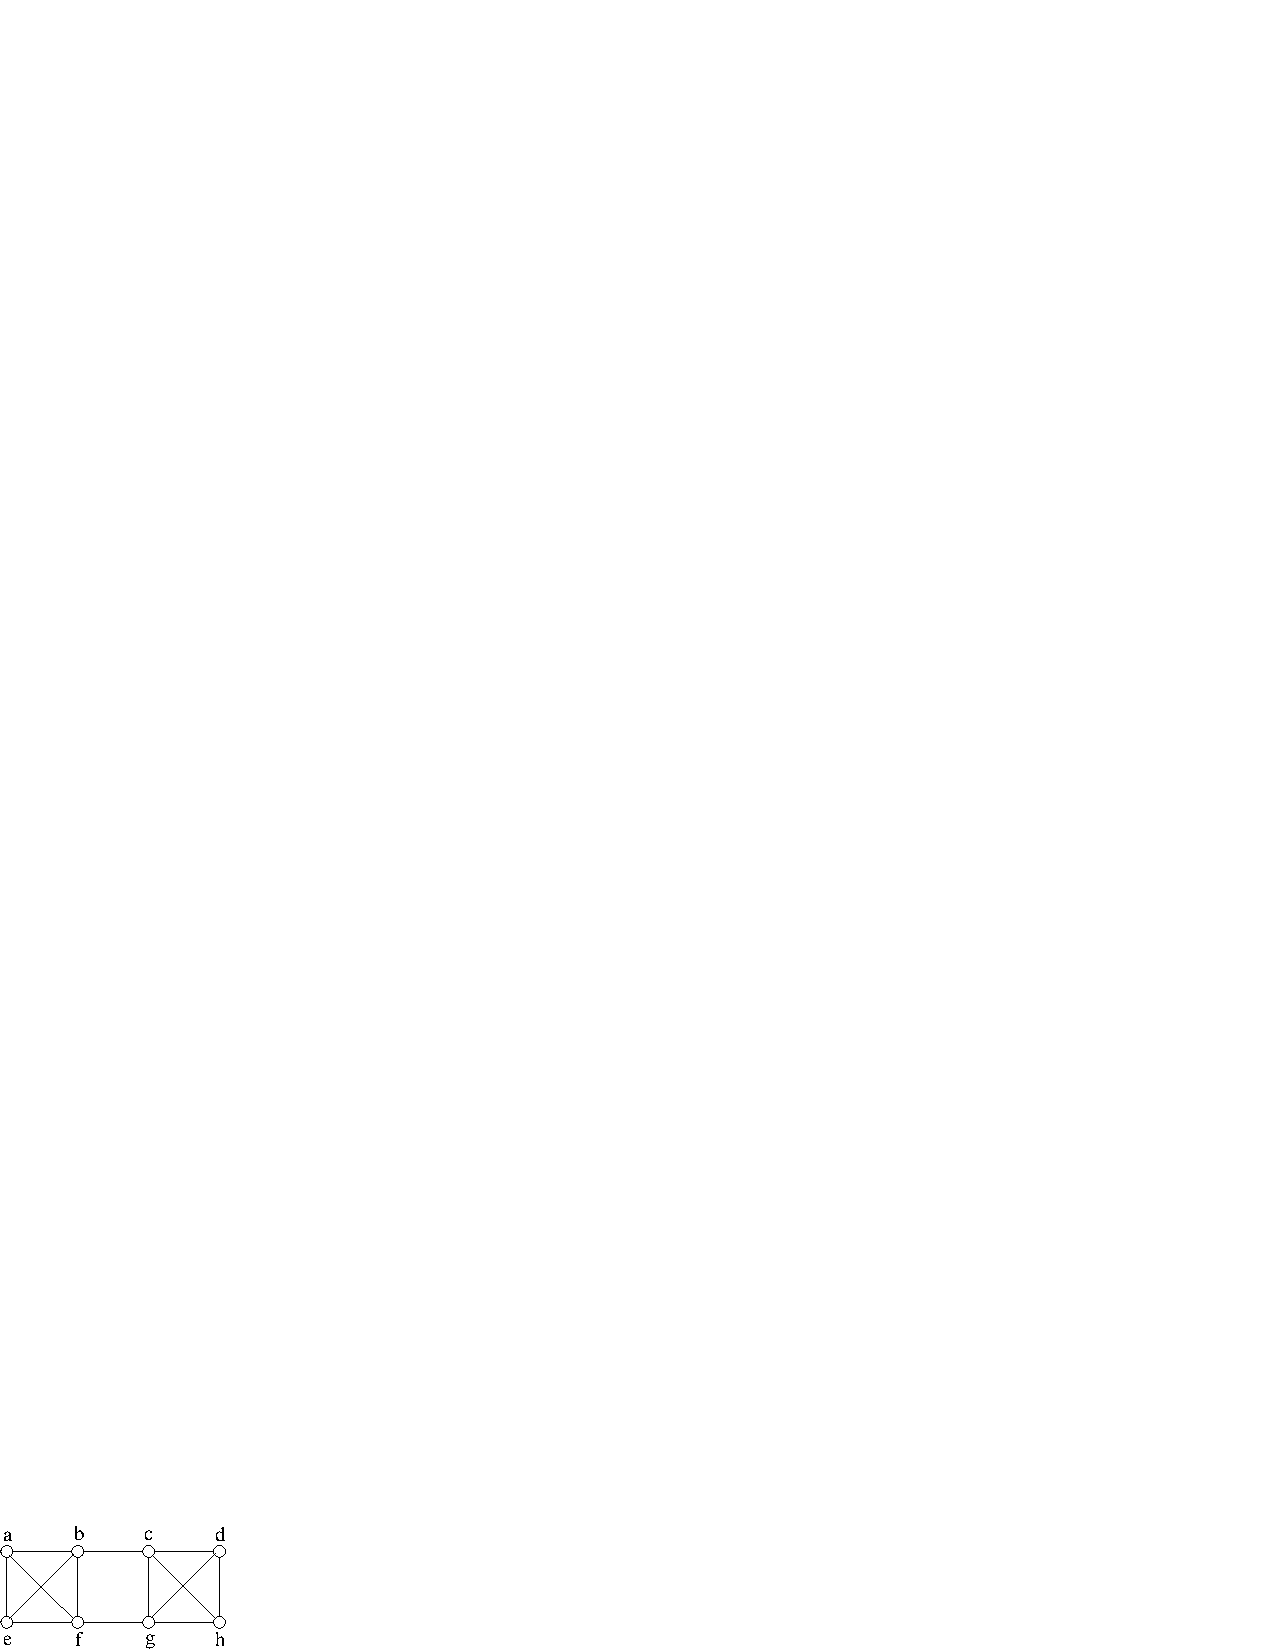
\includegraphics[width=1.5in]{figs/mincut.pdf}
\end{center}

\subsection{Karger's algorithm}

Here's a randomized algorithm for finding the minimum cut:

\begin{itemize}
\item Repeat until just two nodes remain:
\begin{itemize}
\item Pick an edge of $G$ at random and collapse its two endpoints into a single node
\end{itemize}
\item For the two remaining nodes $u_1$ and $u_2$, set 
$V_1 = \{\mbox{nodes that went into $u_1$}\}$ and 
$V_2 = \{\mbox{nodes in $u_2$}\}$
\end{itemize}
An example is shown in Figure~\ref{fig:karger}. Notice
how some nodes end up having multiple edges between them.

\begin{figure}
\begin{center}
\begin{tabular}{cp{.25in}p{2.5in}} \\ \hline

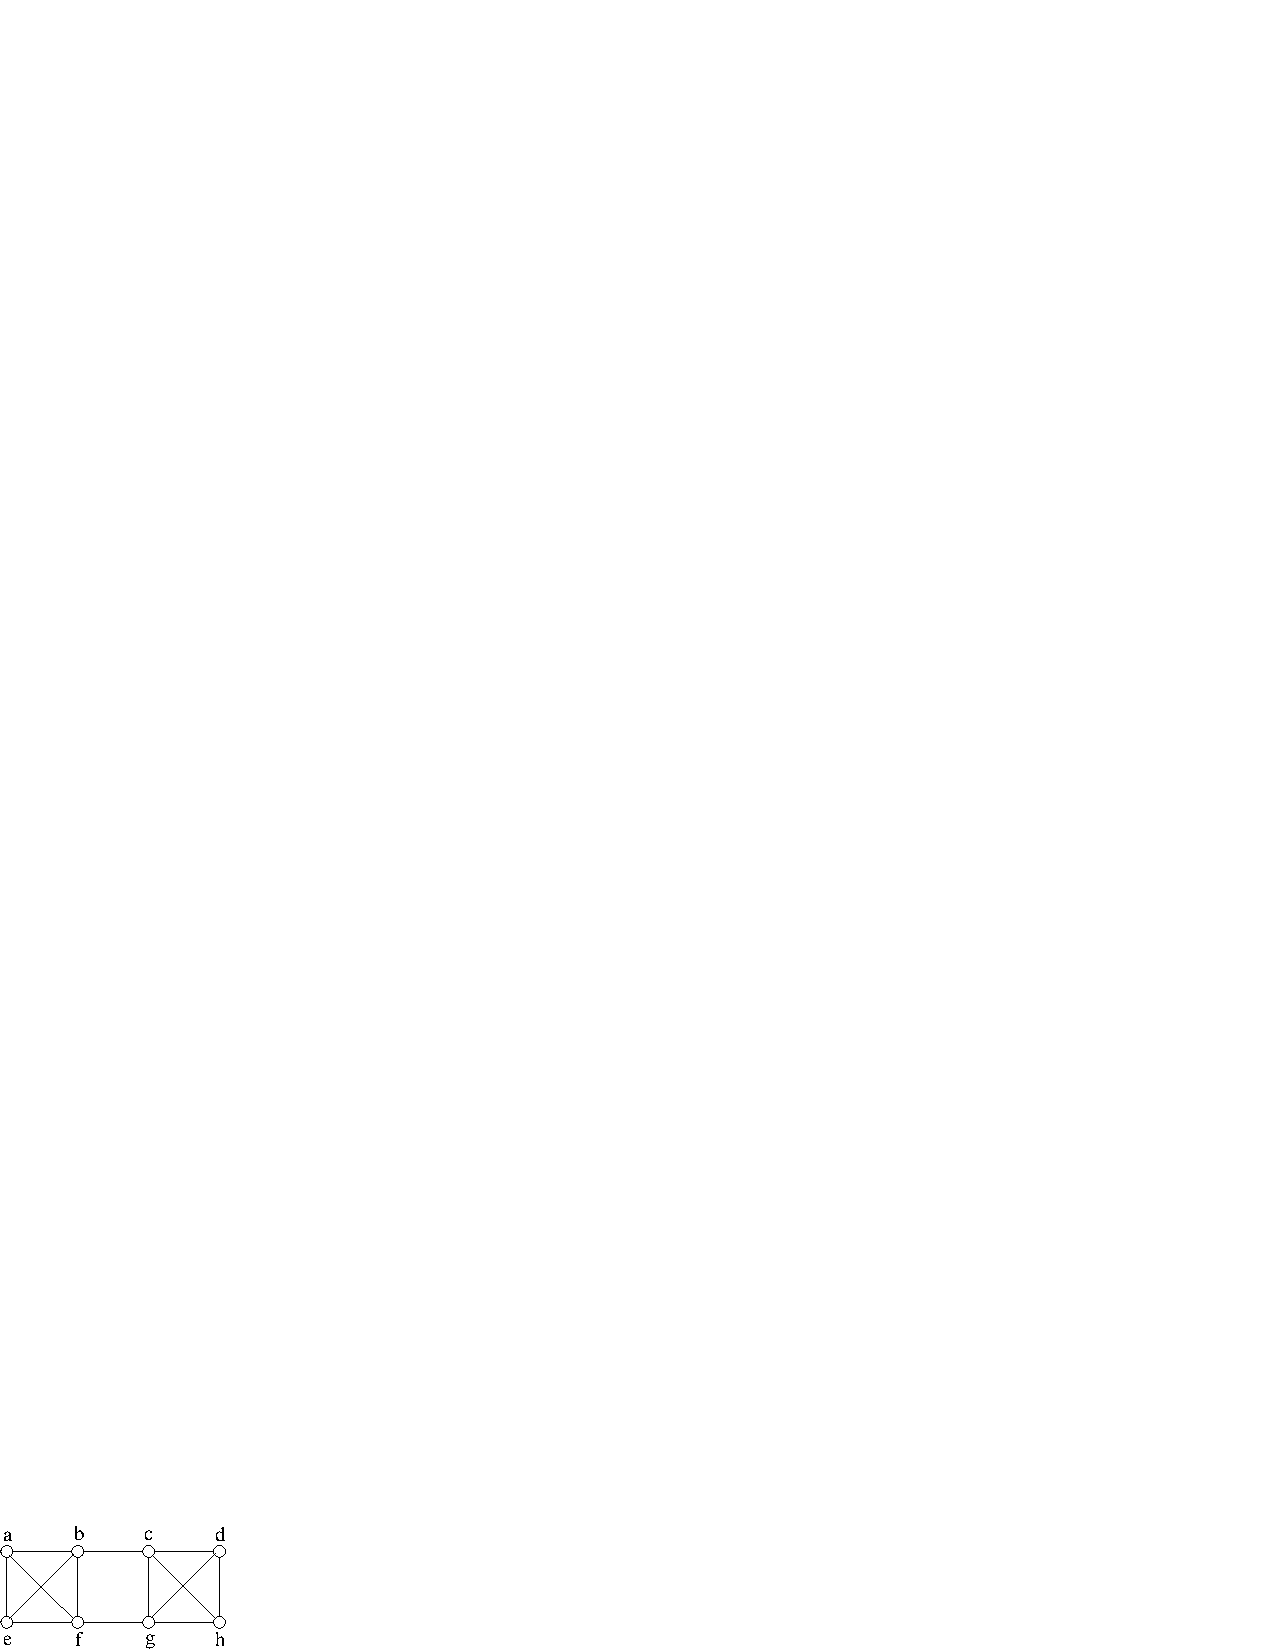
\includegraphics[width=1.5in]{figs/mincut.pdf}
&
&
\raisebox{.4in}
{\begin{minipage}[c]{2.5in}
14 edges to choose from \\
Pick $b-f$ (probability $1/14$)
\end{minipage}}
\\ \hline

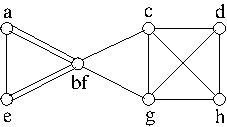
\includegraphics[width=1.5in]{figs/cut1.pdf}
&
&
\raisebox{.4in}
{\begin{minipage}[c]{2.5in}
13 edges to choose from \\
Pick $g-h$ (probability $1/13$)
\end{minipage}}
\\ \hline

\includegraphics[width=1.5in]{figs/cut2.pdf}
&
&
\raisebox{.4in}
{\begin{minipage}[c]{2.5in}
12 edges to choose from \\
Pick $d-gh$ (probability $1/6$)
\end{minipage}}
\\ \hline

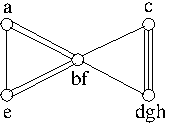
\includegraphics[width=1.25in]{figs/cut3.pdf}
&
&
\raisebox{.4in}
{\begin{minipage}[c]{2.5in}
10 edges to choose from \\
Pick $a-e$ (probability $1/10$)
\end{minipage}}
\\ \hline

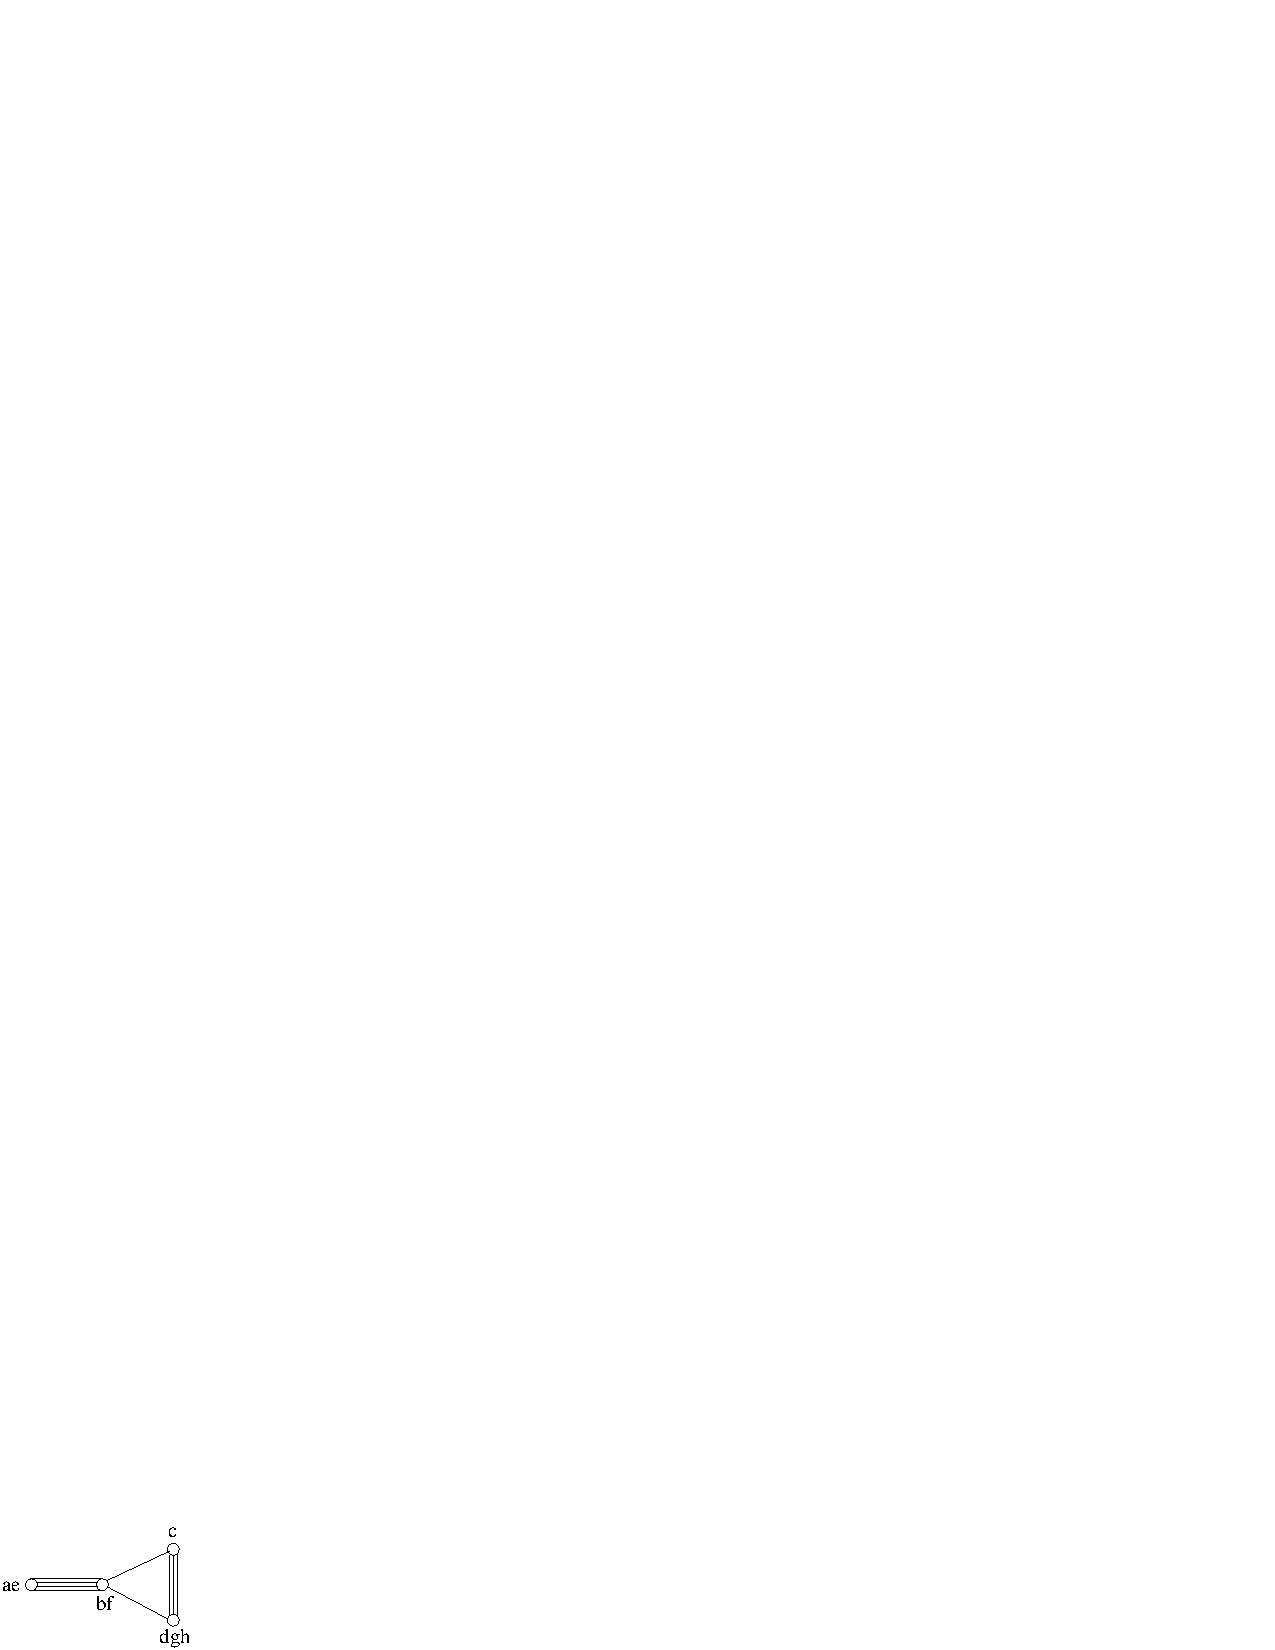
\includegraphics[width=1.35in]{figs/cut4.pdf}
&
&
\raisebox{.4in}
{\begin{minipage}[c]{2.5in}
9 edges to choose from \\
Pick $ab-ef$ (probability $4/9$)
\end{minipage}}
\\ \hline

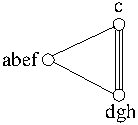
\includegraphics[width=1in]{figs/cut5.pdf}
&
&
\raisebox{.4in}
{\begin{minipage}[c]{2.5in}
5 edges to choose from \\
Pick $c-dgh$ (probability $3/5$)
\end{minipage}}
\\ \hline


\includegraphics[width=1.25in]{figs/cut6.pdf}
&
&
\raisebox{.05in}
{\begin{minipage}[c]{2.5in}
Done: just two nodes remain
\end{minipage}}
\\ \hline
\end{tabular}
\end{center}
\caption{Karger's algorithm at work.}
\label{fig:karger}
\end{figure}



\subsection{Analysis}

Karger's algorithm returns the minimum cut with a certain probability. To analyze it,
let's go through a succession of key facts.

\begin{fact}
If $\mbox{degree}(u)$ denotes the number of edges touching node $u$, then
$$ \sum_{u \in V} \mbox{degree}(u) = 2|E|.$$
\end{fact}
To see this, imagine the following experiment: for each node, list all the edges touching 
it. The number of edges in this list is exactly the left-hand sum. But each edge appears 
exactly twice in it, once for each endpoint.

\begin{fact}
If there are $n$ nodes, then the average degree of a node is $2|E|/n$.
\end{fact}
This is a straightforward calculation: when you pick a node $X$ at random,
$$ 
\E[\mbox{degree}(X)] 
\ = \ 
\sum_{u \in V} \pr(X = u) \mbox{degree}(u) 
\ = \ 
\frac{1}{n} \sum_u \mbox{degree}(u) 
\ = \ 
\frac{2|E|}{n}
$$
where the last step uses the first Fact.

\begin{fact}
The size of the minimum cut is at most $2|E|/n$.
\end{fact}
Consider the partition of $V$ into two pieces, one containing a single node $u$, and the 
other containing the remaining $n-1$ nodes. The size of this cut is $\mbox{degree}(u)$.
Since this is a valid cut, the minimum cut cannot be bigger than this. In other words,
for all nodes $u$,
$$ \mbox{(size of minimum cut)} \leq \mbox{degree}(u) .$$
This means that the size of the minimum cut is also $\leq$ the average degree, which 
we've seen is $2|E|/n$.

\begin{fact}
If an edge is picked at random, the probability that it lies across the minimum cut is 
at most $2/n$.
\end{fact}
This is because there are $|E|$ edges to choose from, and at most $2|E|/n$ of them are
in the minimum cut.
\\

Now we have all the information we need to analyze Karger's algorithm. It returns the
right answer {\it as long as it never picks an edge across the minimum cut}. If it always 
picks a non-cut edge, then this edge will connect two nodes on the same side of the cut,
and so it is okay to collapse them together.

Each time an edge is collapsed, the number of nodes decreases by 1. Therefore,
\begin{eqnarray*}
\pr(\mbox{final cut is the minimum cut})
& = &
\pr(\mbox{first selected edge is not in mincut}) \times \\
& & \pr(\mbox{second selected edge is not in mincut}) \times \cdots \\
& \geq & 
\left( 1 - \frac{2}{n} \right) \left( 1 - \frac{2}{n-1} \right) 
\left( 1 - \frac{2}{n-2} \right) \cdots \left( 1 - \frac{2}{4} \right) 
\left( 1 - \frac{2}{3} \right) \\
& = & 
\frac{n-2}{n} \cdot \frac{n-3}{n-1} \cdot \frac{n-4}{n-2} \cdots \frac{2}{4} \cdot 
\frac{1}{3} \\
& = & 
\frac{2}{n(n-1)} .
\end{eqnarray*}
The last equation comes from noticing that almost every numerator cancels with the 
denominator two fractions down the line.

Karger's algorithm succeeds with probabililty $p \geq 2/n^2$. Therefore,
it should be run $\Omega(n^2)$ times, after which the smallest cut found should
be chosen.

Those who are familiar with minimum spanning tree algorithms might be curious to
hear that another way to implement Karger's algorithm is the following:
\begin{itemize}
\item Assign each edge a random weight
\item Run Kruskal's algorithm to get the minimum spanning tree
\item Break the largest edge in the tree to get the two clusters
\end{itemize}
(Do you see why?) Over the decades, the running time of Kruskal's algorithm has 
been thoroughly optimized via special data structures. Now this same technology 
can be put to work for cuts!

\end{document}



